\chapter[Penulisan dengan \LaTeX - INI HANYA TUTORIAL]{Penulisan dengan \LaTeX - INI HANYA TUTORIAL}

\section{Menampilkan Gambar dan Referensi}
Gambar dapat ditampilkan menggunakan lingkungan \texttt{figure} dan dapat dirujuk menggunakan label. Hasilnya adalah terlihat seperti pada \figref{fig:kucing-example}.

\begin{figure}[H]
    \centering
    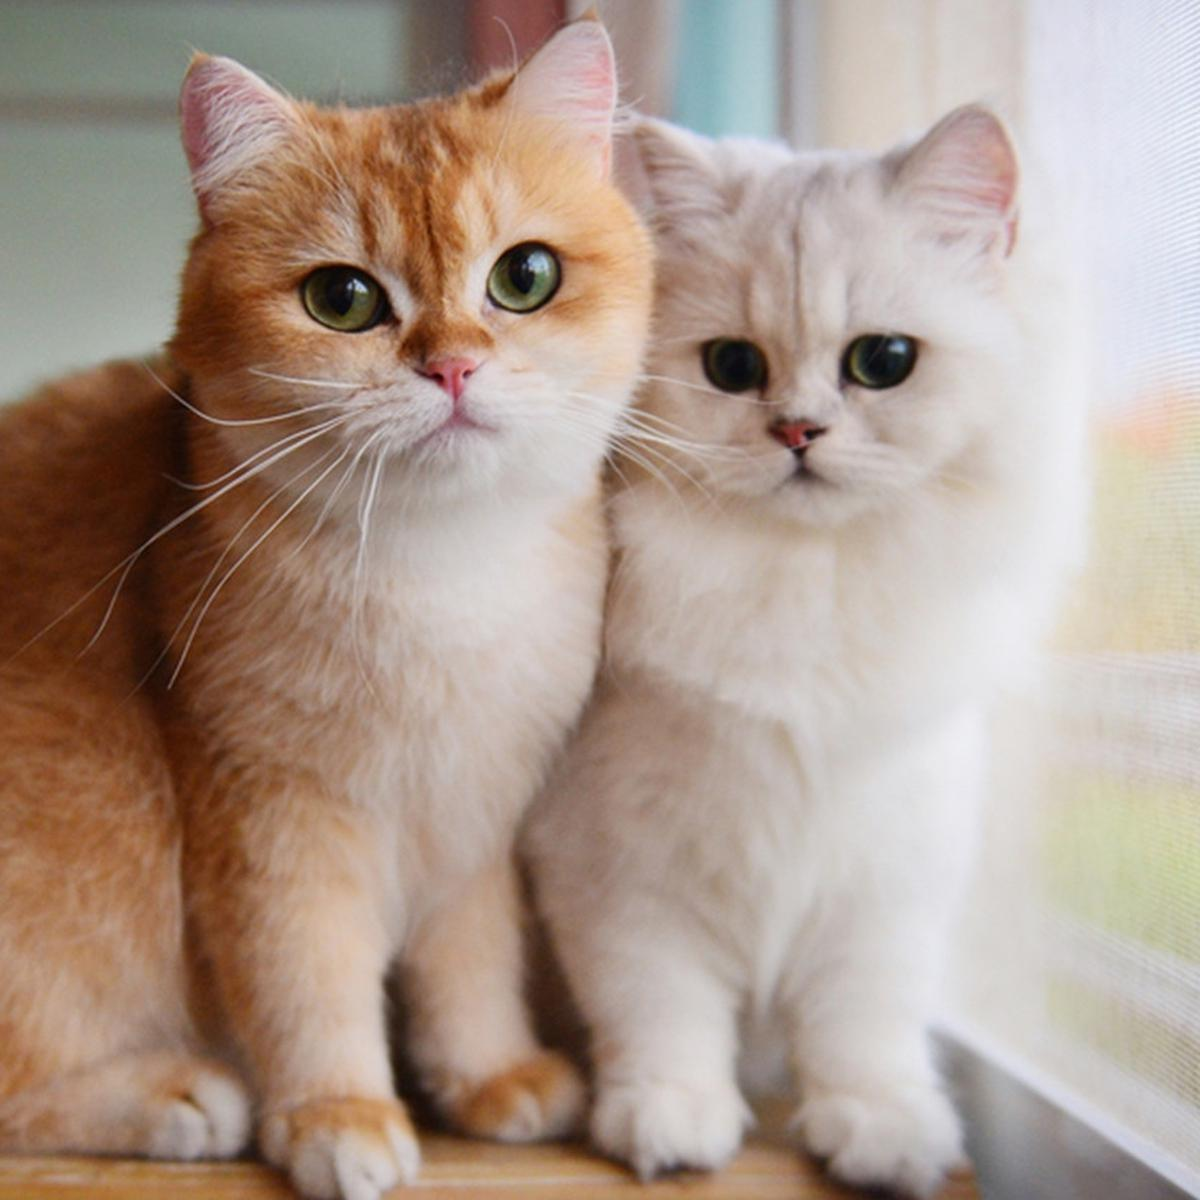
\includegraphics[scale=0.1]{gambar-kucing}
    \caption{Gambar Kucing Lucu dan Imut dengan scala 0.1}
    \label{fig:kucing-example}
\end{figure}

Setiap gambar harus dimention atau disebutkan didalam bacaan seperti contoh di atas. Berikut ini \figref{fig:kucing-example} dan referensi gambar lainnya.

\section{Membuat List atau Daftar}
Terdapat 2 cara yaitu dengan list yang terdapat penomoran 1,2,3 dst atau dengan bullet poin. Secara detail dapat dibaca di bawah.
\subsection{List atau Daftar dengan \texttt{packed\_enum}}
Lingkungan \texttt{packed\_enum} digunakan untuk membuat daftar bernomor dengan jarak yang lebih rapat antar item. Ini sangat berguna untuk menampilkan langkah atau tahapan yang memiliki urutan. Berikut adalah contoh penggunaannya:

\begin{lstlisting}
    \begin{packed_enum}
        \item Langkah pertama adalah mengidentifikasi masalah yang ingin diselesaikan.
        \item Langkah kedua melibatkan analisis kebutuhan.
        \item Langkah ketiga adalah mengembangkan ide dan solusi alternatif.
        \item Langkah keempat adalah melakukan pengujian awal untuk mengevaluasi performa.
    \end{packed_enum}
\end{lstlisting}
    
Hasilnya akan tampak seperti berikut:
\begin{packed_enum}
    \item Langkah pertama adalah mengidentifikasi masalah yang ingin diselesaikan.
    \item Langkah kedua melibatkan analisis kebutuhan.
    \item Langkah ketiga adalah mengembangkan ide dan solusi alternatif.
    \item Langkah keempat adalah melakukan pengujian awal untuk mengevaluasi performa.
\end{packed_enum}

\subsection{List atau Daftar dengan \texttt{packed\_item}}
Lingkungan \texttt{packed\_item} digunakan untuk membuat daftar berpoin dengan jarak antar item yang lebih rapat, cocok untuk poin-poin yang tidak memerlukan urutan tertentu. Berikut adalah contoh penggunaannya:

\begin{lstlisting}
    \begin{packed_item}
        \item Meningkatkan kualitas sensor untuk akurasi yang lebih baik.
        \item Menambahkan modul komunikasi untuk kontrol jarak jauh.
        \item Mengoptimalkan kode untuk efisiensi.
        \item Menambah fitur penghematan energi.
    \end{packed_item}
\end{lstlisting}

Hasilnya akan tampak seperti berikut:
\begin{packed_item}
    \item Meningkatkan kualitas sensor untuk akurasi yang lebih baik.
    \item Menambahkan modul komunikasi untuk kontrol jarak jauh.
    \item Mengoptimalkan kode untuk efisiensi.
    \item Menambah fitur penghematan energi.
\end{packed_item}

\section{Menuliskan Kode Program dengan Listing}
Lingkungan \texttt{lstlisting} memungkinkan kita untuk menuliskan atau menyisipkan kode Python, C++, Arduino, Java atau lainnya dalam dokumen LaTeX dengan format yang rapi dan terstruktur. Pada bagian ini, kita akan melihat dua cara untuk menuliskan kode Python: secara langsung di dalam dokumen dan dengan mengambil dari file eksternal.

\subsection{Kode Python Langsung}

\Lstref{lst:python-direct} menunjukkan fungsi Python yang menghitung faktorial dari sebuah angka. Kode ini ditulis langsung di dalam dokumen LaTeX menggunakan lingkungan \texttt{lstlisting} dengan format diawali dengan \texttt{\textbackslash begin\{lstlisting\}[language=Python, caption=Contoh Kode Python Langsung, label=lst:python-direct]} dan diakhiri dengan \texttt{\textbackslash end\{lstlisting\}}, dimana:
\begin{packed_item}
    \item \texttt{language=Python}: Mengatur pewarnaan sintaksis untuk Python.
    \item \texttt{caption}: Menambahkan keterangan di atas kode untuk menjelaskan isi kode.
    \item \texttt{label}: Menambahkan label untuk memudahkan referensi kode dalam dokumen.
\end{packed_item}

\begin{lstlisting}[language=Python, caption=Contoh Kode Python Langsung, label=lst:python-direct]
def factorial(n):
    if n == 0:
        return 1
    else:
        return n * factorial(n-1)

# Contoh penggunaan
print(factorial(5))  # Output: 120
\end{lstlisting}

\subsection{Kode Python dari File Eksternal}

Jika Anda memiliki file kode Python di folder tertentu (misalnya, di \texttt{kode/code\_sample.py}), Anda bisa menyisipkan kode tersebut langsung ke dalam dokumen LaTeX menggunakan perintah \texttt{\textbackslash lstinputlisting}. Berikut \lstref{lst:python-file} dengan format penulisan \texttt{\textbackslash lstinputlisting[language=Python, caption=Contoh Kode Python dari File, label=lst:python-file]\{kode/code\_sample.py\}}, dimana:
\begin{packed_item}
    \item \texttt{language=Python}: Mengatur pewarnaan sintaksis untuk Python.
    \item \texttt{caption}: Menambahkan keterangan untuk kode yang diambil dari file.
    \item \texttt{label}: Menambahkan label untuk referensi.
    \item \texttt{\{kode/code\_sample.py\}}: Menentukan path atau lokasi file Python yang akan disisipkan. Pastikan file berada di dalam folder \texttt{kode} atau path yang sesuai.
\end{packed_item}

\lstinputlisting[language=Python, caption=Contoh Kode Python dari File, label=lst:python-file]{kode/code_sample.py}

\section{Menambahkan Gambar}
Untuk menambahkan gambar hal yang harus dilakukan adalah:
\begin{packed_enum}
    \item Menyalin file gambar (dalam format jpg \/ png) ke dalam folder \textit{gambar}
    \item Mengganti nama file dari gambar agar mudah dikenali, jangan diberi nama gambar-1,-2, dst
    \item Memasukkan seperti \lstref{lst:kode-gambar}
\end{packed_enum}

\begin{lstlisting}[caption=Kode untuk Menyisipkan Gambar dalam Dokumen, label=lst:kode-gambar]
\begin{figure}[H]
    \centering
    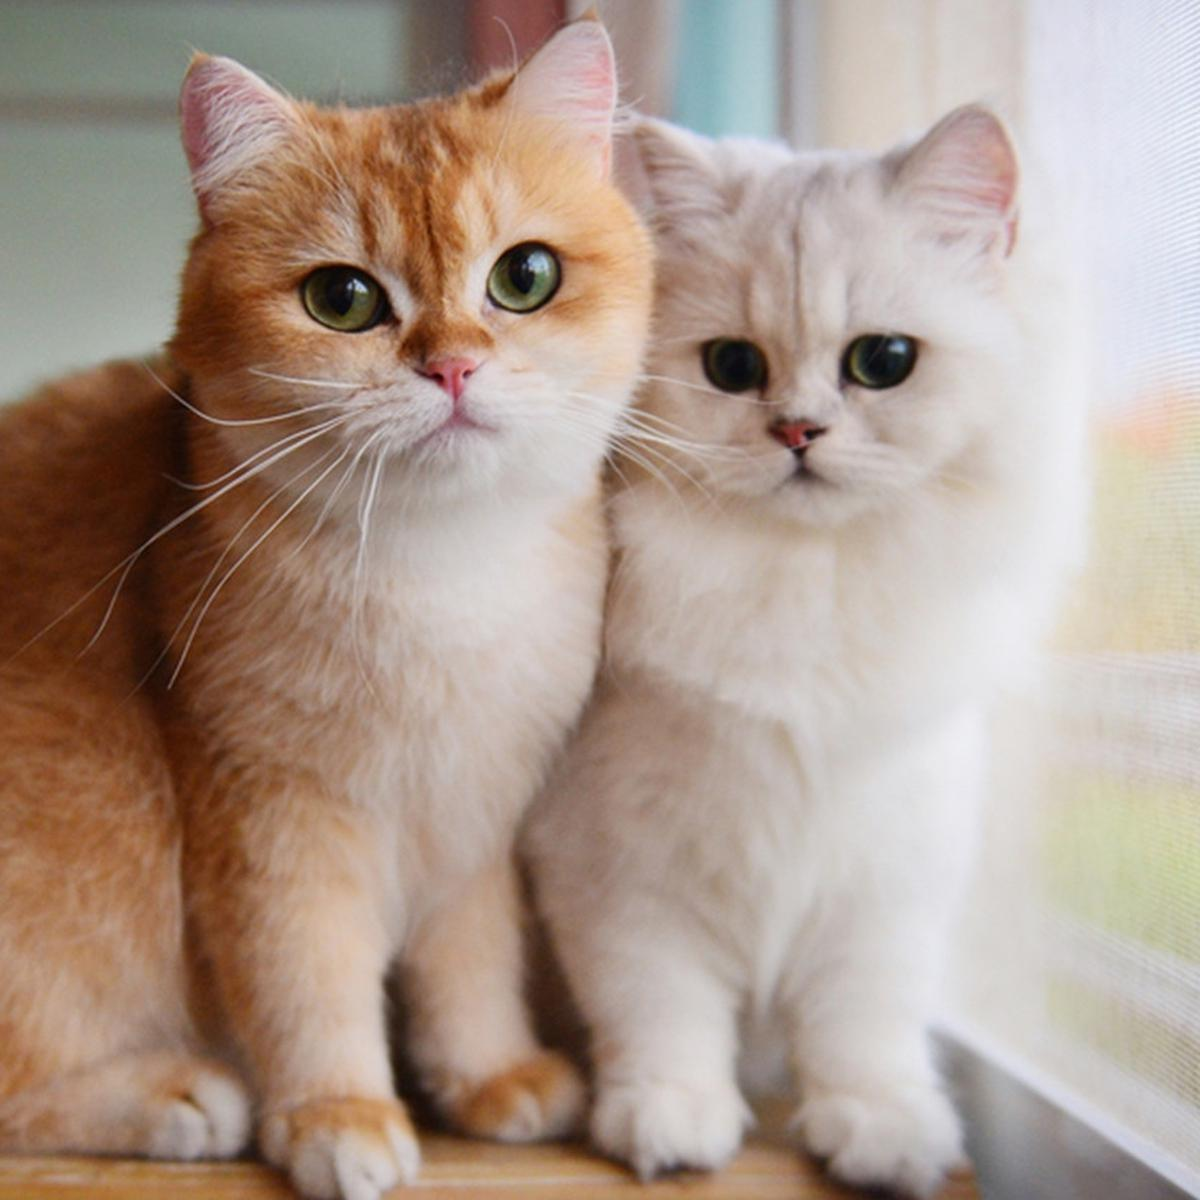
\includegraphics[scale=0.2]{gambar-kucing.jpg}
    \caption{Gambar Kucing Lucu dan Imut}
    \label{fig:nama-gambar}
\end{figure}
\end{lstlisting}

\noindent Berikut adalah penjelasan dari setiap baris pada kode di atas:

\begin{packed_enum}
    \item \texttt{\textbackslash begin\{figure\}[H] ... \textbackslash end\{figure\}}: Membuat lingkungan \texttt{figure} untuk menyisipkan gambar. Parameter \texttt{[H]} digunakan agar gambar diletakkan tepat di posisi yang ditentukan dalam kode. Opsi \textit{H} dapat diganti dengan \textit{h, t, b, p} sesuai kebutuhan.
    \item \texttt{\textbackslash centering}: Mengatur gambar agar berada di tengah halaman.
    \item \texttt{\textbackslash includegraphics[scale=0.2]\{gambar-kucing.jpg\}}: Memasukkan gambar dengan nama file \texttt{gambar-kucing.jpg}. Parameter \texttt{scale=0.2} mengatur ukuran gambar pada 20\% dari ukuran aslinya. Ubah nilainya untuk memperbesar atau memperkecil gambar.
    \item \texttt{\textbackslash caption\{Gambar Kucing Lucu dan Imut\}}: Menambahkan keterangan (caption) di bawah gambar yang akan muncul di Daftar Gambar dan disertai nomor gambar secara otomatis.
    \item \texttt{\textbackslash label\{fig:kucing\}}: Memberikan label pada gambar untuk merujuk gambar ini dalam teks menggunakan \texttt{\textbackslash figref\{fig:kucing\}} atau \texttt{\textbackslash ref\{fig:kucing\}} yang menghasilkan "gambar 1" atau penomoran gambar sesuai urutan.
\end{packed_enum}

Hasilnya adalah terlihat seperti pada \figref{fig:kucing-demo}.

\begin{figure}[H]
    \centering
    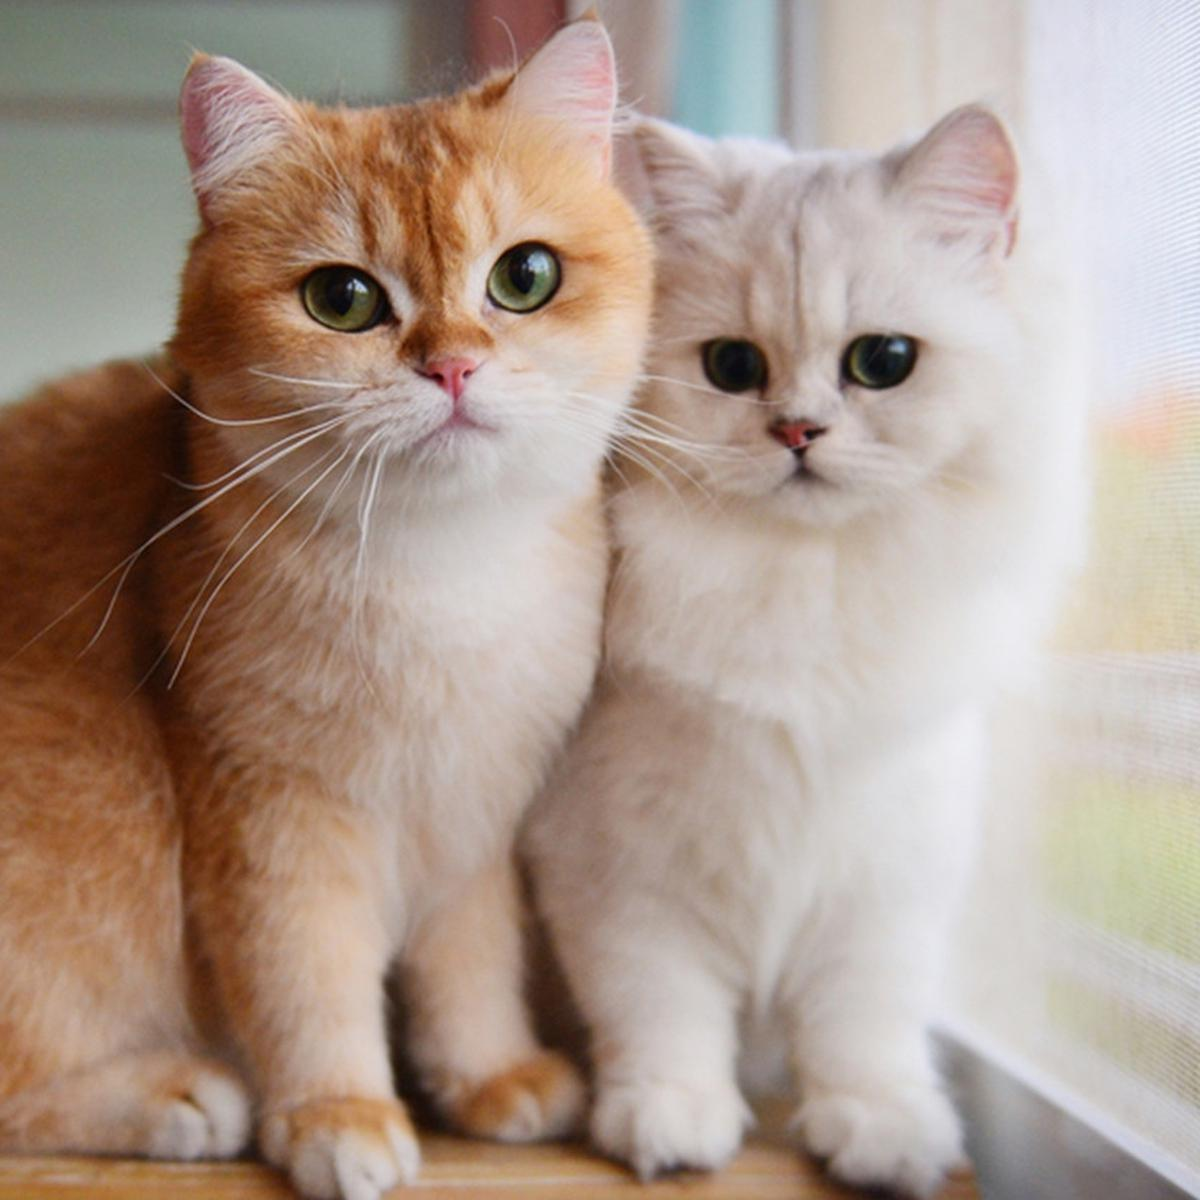
\includegraphics[scale=0.1]{gambar-kucing}
    \caption{Gambar Kucing Lucu dan Imut dengan scala 0.1}
    \label{fig:kucing-demo}
\end{figure}

Setiap gambar harus dimention atau disebutkan didalam bacaan seperti berikut ini \figref{fig:kucing-demo} dan \figref{fig:logoUNY}.

\begin{figure}[H]
    \centering
    
\includegraphics[scale=0.4]{logo-uny}
    \caption{Logo UNY dengan scala 0.4}
    \label{fig:logoUNY}
\end{figure}

\section{Membuat Tabel}
Tabel dalam LaTeX dapat dibuat menggunakan lingkungan \texttt{table} dan \texttt{tabular}. Tabel sangat berguna untuk menyajikan data secara terstruktur dan mudah dibaca. Berikut ini adalah contoh pembuatan tabel sederhana dan tabel yang lebih kompleks.

\subsection{Tabel Sederhana}
\Tabref{tab:contoh-sederhana} menunjukkan contoh tabel sederhana dengan data hasil pengujian. Tabel ini menggunakan format dasar dengan garis pembatas horizontal dan vertikal.

\begin{table}[H]
    \centering
    \caption{Hasil Pengujian Sensor}
    \label{tab:contoh-sederhana}
    \begin{tabular}{|c|c|c|}
        \hline
        \textbf{No} & \textbf{Sensor} & \textbf{Akurasi (\%)} \\
        \hline
        1 & DHT22 & 95.2 \\
        \hline
        2 & BMP280 & 98.5 \\
        \hline
        3 & MPU6050 & 92.8 \\
        \hline
        4 & HC-SR04 & 89.7 \\
        \hline
    \end{tabular}
\end{table}

\subsection{Tabel dengan Format Lanjutan}
\Tabref{tab:perbandingan-metode} menunjukkan contoh tabel yang lebih kompleks dengan penggabungan kolom dan baris. Tabel ini menggunakan paket \texttt{multirow} untuk menggabungkan sel.

\begin{table}[H]
    \centering
    \caption{Perbandingan Metode Pembelajaran Mesin}
    \label{tab:perbandingan-metode}
    \begin{tabular}{|l|c|c|c|c|}
        \hline
        \multirow{2}{*}{\textbf{Metode}} & \multicolumn{2}{c|}{\textbf{Dataset A}} & \multicolumn{2}{c|}{\textbf{Dataset B}} \\
        \cline{2-5}
        & \textbf{Akurasi} & \textbf{Waktu (s)} & \textbf{Akurasi} & \textbf{Waktu (s)} \\
        \hline
        Random Forest & 94.2\% & 12.5 & 91.8\% & 15.3 \\
        \hline
        SVM & 92.6\% & 8.7 & 89.4\% & 11.2 \\
        \hline
        Neural Network & 96.1\% & 45.8 & 94.7\% & 52.1 \\
        \hline
        Decision Tree & 88.9\% & 3.2 & 85.6\% & 4.1 \\
        \hline
    \end{tabular}
\end{table}

\subsection{Penjelasan Pembuatan Tabel}
Berikut adalah penjelasan dari komponen-komponen pembuat tabel:

\begin{packed_enum}
    \item \texttt{\textbackslash begin\{table\}[H] ... \textbackslash end\{table\}}: Membuat lingkungan \texttt{table} untuk tabel. Parameter \texttt{[H]} digunakan agar tabel diletakkan tepat di posisi yang ditentukan.
    \item \texttt{\textbackslash centering}: Mengatur tabel agar berada di tengah halaman.
    \item \texttt{\textbackslash caption\{...\}}: Menambahkan judul tabel yang akan muncul di Daftar Tabel.
    \item \texttt{\textbackslash label\{tab:...\}}: Memberikan label pada tabel untuk referensi menggunakan \texttt{\textbackslash tabref\{tab:...\}}.
    \item \texttt{\textbackslash begin\{tabular\}\{|c|c|c|\}}: Mendefinisikan struktur kolom tabel, dimana \texttt{c} = center, \texttt{l} = left, \texttt{r} = right, dan \texttt{|} = garis vertikal.
    \item \texttt{\textbackslash hline}: Membuat garis horizontal.
    \item \texttt{\textbackslash multirow\{2\}\{*\}\{teks\}}: Menggabungkan beberapa baris dalam satu kolom.
    \item \texttt{\textbackslash multicolumn\{2\}\{c|\}\{teks\}}: Menggabungkan beberapa kolom dalam satu baris.
    \item \texttt{\textbackslash cline\{2-5\}}: Membuat garis horizontal hanya pada kolom 2-5.
\end{packed_enum}

Referensi tabel dapat dilakukan dengan mudah seperti ini: "Berdasarkan data pada \tabref{tab:contoh-sederhana}, sensor BMP280 memiliki akurasi tertinggi", atau "Seperti yang ditunjukkan pada \tabref{tab:perbandingan-metode}, Neural Network memberikan hasil terbaik."

\section{Menggambar dengan TikZ}
TikZ adalah salah satu paket LaTeX yang sangat powerful untuk membuat diagram, grafik, dan ilustrasi teknis. TikZ memungkinkan pembuatan gambar vektor yang presisi dan dapat diintegrasikan sempurna dengan teks LaTeX. Pada bagian ini, kita akan melihat beberapa contoh penggunaan TikZ untuk membuat berbagai jenis gambar.

\subsection{Diagram Sederhana}
\Figref{fig:tikz-simple} menunjukkan contoh diagram sederhana menggunakan TikZ. Diagram ini menunjukkan proses alur kerja sistem dengan menggunakan bentuk-bentuk dasar dan panah.

\begin{figure}[H]
    \centering
    \begin{tikzpicture}[node distance=2cm, auto]
        % Define styles
        \tikzstyle{startstop} = [rectangle, rounded corners, minimum width=3cm, minimum height=1cm, text centered, draw=black, fill=red!30]
        \tikzstyle{process} = [rectangle, minimum width=3cm, minimum height=1cm, text centered, draw=black, fill=orange!30]
        \tikzstyle{decision} = [diamond, minimum width=3cm, minimum height=1cm, text centered, draw=black, fill=green!30]
        \tikzstyle{arrow} = [thick,->,>=stealth]
        
        % Draw nodes
        \node (start) [startstop] {Start};
        \node (input) [process, below of=start] {Input Data};
        \node (process1) [process, below of=input] {Process Data};
        \node (decision1) [decision, below of=process1, yshift=-0.5cm] {Valid?};
        \node (output) [process, below of=decision1, yshift=-0.5cm] {Output Result};
        \node (stop) [startstop, below of=output] {End};
        \node (error) [process, right of=decision1, xshift=2cm] {Show Error};
        
        % Draw arrows
        \draw [arrow] (start) -- (input);
        \draw [arrow] (input) -- (process1);
        \draw [arrow] (process1) -- (decision1);
        \draw [arrow] (decision1) -- node[anchor=east] {Yes} (output);
        \draw [arrow] (decision1) -- node[anchor=south] {No} (error);
        \draw [arrow] (error) |- (input);
        \draw [arrow] (output) -- (stop);
    \end{tikzpicture}
    \caption{Diagram Alur Kerja Sistem dengan TikZ}
    \label{fig:tikz-simple}
\end{figure}

\subsection{Grafik dan Plot}
TikZ juga dapat digunakan untuk membuat grafik matematika dan plot data. \Figref{fig:tikz-plot} menunjukkan contoh grafik fungsi matematika yang dibuat menggunakan pgfplots, yang merupakan bagian dari TikZ.

\begin{figure}[H]
    \centering
    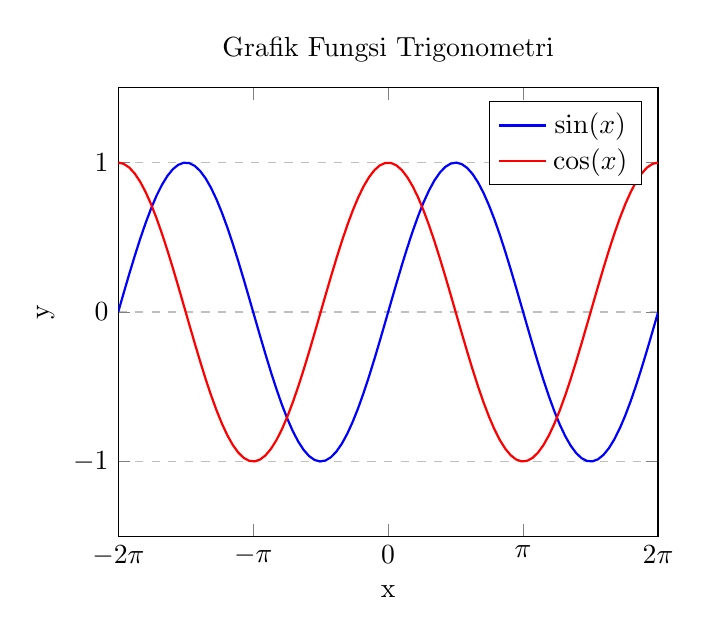
\begin{tikzpicture}
        \begin{axis}[
            title={Grafik Fungsi Trigonometri},
            xlabel={x},
            ylabel={y},
            xmin=-6.28, xmax=6.28,
            ymin=-1.5, ymax=1.5,
            xtick={-6.28,-3.14,0,3.14,6.28},
            xticklabels={$-2\pi$,$-\pi$,0,$\pi$,$2\pi$},
            ytick={-1,0,1},
            legend pos=north east,
            ymajorgrids=true,
            grid style=dashed,
        ]
        
        \addplot[
            color=blue,
            mark=none,
            samples=100,
            domain=-6.28:6.28,
            thick
        ] {sin(deg(x))};
        \addlegendentry{$\sin(x)$}
        
        \addplot[
            color=red,
            mark=none,
            samples=100,
            domain=-6.28:6.28,
            thick
        ] {cos(deg(x))};
        \addlegendentry{$\cos(x)$}
        
        \end{axis}
    \end{tikzpicture}
    \caption{Grafik Fungsi Sinus dan Cosinus}
    \label{fig:tikz-plot}
\end{figure}

\subsection{Diagram Blok Sistem}
\Figref{fig:tikz-block} menampilkan diagram blok sistem kontrol yang umum digunakan dalam teknik. Diagram ini menunjukkan hubungan antara komponen-komponen sistem.

\begin{figure}[H]
    \centering
    \begin{tikzpicture}[auto, node distance=2cm, >=stealth']
        % Define block styles
        \tikzstyle{block} = [draw, fill=blue!20, rectangle, minimum height=3em, minimum width=6em]
        \tikzstyle{sum} = [draw, fill=blue!20, circle, node distance=1cm]
        \tikzstyle{input} = [coordinate]
        \tikzstyle{output} = [coordinate]
        \tikzstyle{pinstyle} = [pin edge={to-,thin,black}]
        
        % Place nodes
        \node [input, name=input] {};
        \node [sum, right of=input] (sum) {};
        \node [block, right of=sum] (controller) {Controller};
        \node [block, right of=controller, node distance=3cm] (system) {Plant/System};
        \node [output, right of=system] (output) {};
        \node [block, below of=system] (sensor) {Sensor};
        
        % Draw connections
        \draw [->] (input) -- node {$r(t)$} (sum);
        \draw [->] (sum) -- node {$e(t)$} (controller);
        \draw [->] (controller) -- node {$u(t)$} (system);
        \draw [->] (system) -- node [name=y] {$y(t)$} (output);
        \draw [->] (y) |- (sensor);
        \draw [->] (sensor) -| node[pos=0.99] {$-$} node [near end] {$y_m(t)$} (sum);
        
        % Labels
        \draw [->] (input) -- node[above] {Reference} +(-1,0);
        \draw [->] (output) -- node[above] {Output} +(1,0);
    \end{tikzpicture}
    \caption{Diagram Blok Sistem Kontrol Feedback}
    \label{fig:tikz-block}
\end{figure}

\subsection{Diagram Jaringan}
\Figref{fig:tikz-network} menunjukkan contoh diagram jaringan yang dapat digunakan untuk menggambarkan topologi jaringan komputer atau arsitektur sistem.

\begin{figure}[H]
    \centering
    \begin{tikzpicture}[
        node distance=3cm,
        server/.style={rectangle, draw, fill=yellow!30, minimum width=2cm, minimum height=1cm},
        client/.style={circle, draw, fill=blue!20, minimum size=1cm},
        router/.style={diamond, draw, fill=orange!30, minimum size=1.5cm}
    ]
        % Server
        \node[server] (server) at (0,0) {Server};
        
        % Router
        \node[router] (router) at (4,0) {Router};
        
        % Clients
        \node[client] (client1) at (7,2) {PC1};
        \node[client] (client2) at (7,0) {PC2};
        \node[client] (client3) at (7,-2) {PC3};
        
        % Internet cloud (simplified as ellipse)
        \node[draw, ellipse, fill=gray!20, minimum width=2cm, minimum height=1cm] (internet) at (-3,0) {Internet};
        
        % Connections
        \draw[thick] (internet) -- (server);
        \draw[thick] (server) -- (router);
        \draw[thick] (router) -- (client1);
        \draw[thick] (router) -- (client2);
        \draw[thick] (router) -- (client3);
        
        % Labels
        \node[above] at ($(internet)!0.5!(server)$) {WAN};
        \node[above] at ($(server)!0.5!(router)$) {LAN};
        \node[above right] at ($(router)!0.5!(client1)$) {Ethernet};
        \node[right] at ($(router)!0.5!(client2)$) {Ethernet};
        \node[below right] at ($(router)!0.5!(client3)$) {Ethernet};
    \end{tikzpicture}
    \caption{Diagram Topologi Jaringan}
    \label{fig:tikz-network}
\end{figure}

\subsection{Pie Chart dengan TikZ}
\Figref{fig:tikz-pie} menampilkan cara membuat pie chart menggunakan paket pgf-pie yang merupakan ekstensi dari TikZ.

\begin{figure}[H]
    \centering
    \begin{tikzpicture}
        \pie[
            text=legend,
            radius=3,
            color={blue!60, red!60, green!60, yellow!60, purple!60}
        ]{
            35/Programming,
            25/Documentation,
            20/Testing,
            15/Analysis,
            5/Others
        }
    \end{tikzpicture}
    \caption{Distribusi Waktu Pengembangan Software}
    \label{fig:tikz-pie}
\end{figure}

\subsection{Tips Penggunaan TikZ}
Berikut adalah beberapa tips penting dalam menggunakan TikZ:

\begin{packed_enum}
    \item \textbf{Perencanaan}: Selalu buat sketsa manual terlebih dahulu sebelum coding dengan TikZ.
    \item \textbf{Koordinat}: Gunakan sistem koordinat yang konsisten dan mudah dipahami.
    \item \textbf{Style}: Definisikan style untuk elemen yang berulang agar kode lebih rapi.
    \item \textbf{Library}: Manfaatkan library TikZ seperti \texttt{positioning}, \texttt{shapes}, \texttt{arrows}, dll.
    \item \textbf{Modularitas}: Pisahkan gambar kompleks menjadi bagian-bagian kecil.
    \item \textbf{Dokumentasi}: Tambahkan komentar pada kode TikZ yang kompleks.
\end{packed_enum}

\begin{packed_item}
    \item \textbf{Shapes Library}: Untuk bentuk-bentuk khusus seperti diamond, ellipse, dll.
    \item \textbf{Positioning Library}: Untuk positioning node yang lebih fleksibel.
    \item \textbf{Arrows Library}: Untuk berbagai jenis panah dan garis.
    \item \textbf{Calc Library}: Untuk kalkulasi koordinat yang kompleks.
    \item \textbf{Patterns Library}: Untuk pola pengisian area.
\end{packed_item}

\section{Referensi dan Sitasi}
Referensi dan sitasi pada dokumen \LaTeX juga cukup mudah. Silahkan buka file \textit{pustaka.bib} dan amati beberapa contoh penulisan referensi yang ada. Untuk menggenerate bentuk referensi seperti ini dapat menggunakan Mendeley atau Zotero. Mensitasi referensi seperti ini \citep{Priambodo_2021}, \citep{Nasuha_2017}, \citep{Dhewa_Dharmawan_Priyambodo_2017}, \citep{Arifin_2015} dapat dilakukan dengan perintah \verb|\citep{nama_label}|. Pemberian sitasi dengan benar membuat sitasi tersebut dapat di klik dan akan mengarahkan ke daftar pustaka.
